\chapter{Overview}
\label{chapterlabel2}
\section{Overview}
%As mentioned previously this report looks to implement convolutional networks for video classification particularly looking at action labelled data.
% explain convultional netweorks with pooling layer
The project begins by constructing convolutional neural networks models using the Keras API and the TensorFlow framework taking as an input a video frames containing an image from the video.
It then moves on to use other architectures that take into account temporal features.
The initial architectures will be based off those discussed in \citep{KarpathyCVPR14}, where different models are explored for large-scale video classification with convolutional neural networks.
These models will be built using the python as the programming language.
This project will also investigate popular pretrained models with the current software and hardware available.
Another aim of the project will be to explore the difficulties with recreating popular models with the current software and hardware at hand.
It also aims to give an understanding from a software engineering perspective on how to begin with constructing these models.
% with the future aim of exploring with emotion classification using image and video data. Something that has been explored in papers such as \cite{SUN201836}
% explain f what a convutional neural network is here, talk about Alexnet
% In order to get familiar with building neural networks, the first task involved  then understanding the structure and looking atthe performance of pretrained models CNN models readily available.



\subsection{Setup}
% todo explain the clusters better
%what is pip
Since the project required TensorFlow and the Keras API with python programming language, python 3.6 was used as it is the newer and more compatible python version from the legacy soon to be deprecated python 2.7.
The initial coding environment set up was done using Anaconda which is a an open-source distribution for python and python libraries which are typically used for scientific computing.
It also provides a distribution for R programming language.
A benefit of anaconda is that it allows for multiple python environments and easy download of libraries and a very friendly user graphical interface as well as a command line interface.
%todo pip and reference
Pip which is the python specific library management tool was also used to download some TensorFlow libraries which were not available in anaconda.

The TensorFlow libraries comes in two distribution the first being the GPU enabled distribution with uses the GPU first by default to speed up certain processes before it uses the CPU.
The second distribution simply runs on the CPU only.
The project initially began on a laptop with no GPU capacity, hence the TensorFlow CPU package was installed. The project al
As mentioned briefly previously, Tensorflow uses a dataflow graph in which the nodes represent units of computation, and the edges represent the input data or the output data of the computation. This data flow allows for benefits such as the use of parallel computing for model, distributed execution through the use of explicit edges which allow for partitioning across multiple devices. It also improves compilation and generates faster code by allowing TensorFlow's XLA compiler use dataflow graph information. The dataflow graph is also language independ allowing for prtability between language.
TensorFlow comes with a keras API within its libraries, this version of Keras supports the use of the datagraph unlike the readily available keras library hence it is there is no need to download keras separately in order to reap the benefits of te Tensorflow data flow.
The project also initially began in a jupyter notebook environment which is an open sourced web-based interactive development environment used for a multitude of scientific research. An Empirical Study on Jupyter notebook as a tool for open science has also been taken as seen in \citep{Randles_2017}. While on jupyter notebook, TensorFlow was ran in eager mode which is a programming environment provided by TensorFlow which evaluates operations from the dataflow graph immediately by not building computational graphs, hence allowing concrete values to be returned instead of constructing a graph to run later making debugging easier in such an interactive environment like jupyter notebook.
Once familiar with the working of the Tensorflow environment, The models when then transferred into python scripts and then ran in the terminal then on the UCL cluster infrastructure using the interactive session, which allows for requesting nodes with different processing configuration. Using this interactive session to decide on what the clock time and hardware will be needed for script when ran in a batch job. The time needed to run each job was approximated based on the time taken for the first steps in the fist epoch from the interactive mode. Computing with GPU, CPU and parallel running we considered.

% Rather building models from scracth the TensorFlow package and keras  packages where used to construct the models and access the pre-trained models.

\subsection{Datasets}
Tensorflow also provides readily available pre-processed data sets for easy use. these datasets are available using the TensorFlow dataset library. The Tensorflow dataset is a library that exposes publicly available datasets as numpy arrays, TensorFlow dataset object and tensors. The range of datasets range from images to audio to text datasets.
This project used the UCF101 dataset provided by this library which is an action recognition data set of realistic action videos, collected from YouTube, having 101 action categories \cite{soomro2012ucf101}. It contains about 13320 videos from 101 action categories, the videos in 101 action categories are grouped into 25 groups, where each group can consist of 4-7 videos of an action, videos from the same group may share some common features, such as similar background, similar viewpoint, etc.
The action categories can be divided into five types which include Human-Object Interaction, Body-Motion Only, Human-Human Interaction , Playing Musical Instruments and Sports.
Tensorflow also provides a train test split of the data where number of training examples are 9537 and the number of test examples are 3783.
It also provides the functionality to take a custom spilt of the data and reduce the number of videos used for training. Each clip contains mutiple frames of 256x256x3.
%todo crosscheck how youtube-8m download works%
This UCF101 data set is also used in \citep{KarpathyCVPR14} to train models based off pretrained models trained with the larger data set of sports-1M validation of the final models trained on the sport-1M dataset.
Although most of links of the videos in the sports-1M dataset, which consists of over one million YouTube videos belonging to about 487 classes of sports is readily available on youtube for download there is a challenge of speed of model and with memory when it comes to downloading this large dataset. There is also the challenge were there is no clear copyright instruction for download applicable to all the videos. Hence the smaller UCF101 was decided to be used to recreate the models. It is also important to note that the sports-1M is also available as part youtube-8M datset. And although there is an API available to download youtube-8M as TensorFlow Record file, the sports-1M dataset cannot be easily separated out of youtube-8M as it does not allow for access to specific videos. which would be a nice addition because the sport-1M dataset github page provides the list of videos included in the sport-1M dataset split into training and test datasets.

% might be worth summaring the dataset used in karpathy's paper


\subsection{Architectures}

In Karpathy paper on Large-scale Video Classification with convolutional Neural Networks \citep{KarpathyCVPR14}, it discusses various models and explores approaches for fusing information over temporal dimension through the convolutional network and compares their performance. Using the UCF101 dataset and TensorFlow, I will also explore recreating these models and apply newer techniques for optimization. The models which will be implemented are listed below. The structures of these models can be also be seen in figure \ref{fig:k_models} taken from \citep{KarpathyCVPR14}
\begin{itemize}
    \item Single Frame: is loosely based on the Alexnet model \cite{NIPS2012_4824}, which was the winning model of the ImageNet challenge in 2012. Alexnet model takes in an input image of $224 \times 224 \times 3$, using the shorthand notation as described in \citep{KarpathyCVPR14}, the full architecture is $C(96, 11, 4)-N-P-C(256, 5, 1)-N-P-C(384, 3, 1)-C(384, 3, 1)-C(256, 3, 1)-P-F C(4096)-F C(4096)$, where $C(d, f, s)$, is a convolutional layer with d filters of spatial size $ f × f$, with a stride of $s$,  $FC(n)$ is a fully connected layer with n nodes, $N$ is local response normalization layer and P is the pooling layer. The single frame model from \cite{KarpathyCVPR14} follows the following architecture  $C(96, 11, 3)-N-P-C(256, 5, 1)-N-P-C(384, 3, 1)-C(384, 3, 1)-C(256, 3, 1)-P-F C(4096)-FC(4096)$ with the exception that it takes in an image of size $ 170 \times 170 \times 3$. The single frame also uses a max pooling is non-overlapping with size $2 \times 2$ rather than overlapping pooling of size $3x3$ and stride $2$ used in the Alexnet. This is an interesting difference that might have an effect on performance as the Alexnet paper suggest that gerrally they observed during training that models with overlapping pooling found it slightly more difficult to overfit.
    \item Early Fusion - This combines information across an entire time window immediately on the pixel level hence making the input size that of $11 \times 11 \times 3 \times T$ pixels, where T was 10 which is also the number of frames covered. The change in input shape also required a change to the first convolutional layer to use a filter size of $10 \times 11 \times 11$.
    \item Late Fusion: This uses two single frame networks, taking in about 15 frames apart and combining them at the fully connected layers
    \item Slow Fusion: Is a mix of both late and early fusion, slowly combing the temporal information over at each convolutional layer. The input is a clip containing 10 frames. The first convolution layer now consist of 4 parallel layers that each take in 4 frames out of this clip, The second convolutional layer consist of two parallel layers that combines the two outputs from the first while the third layer combines the output from the second layer
\end{itemize}

\subsection{assumptions}
some assumptiones



\begin{figure}
    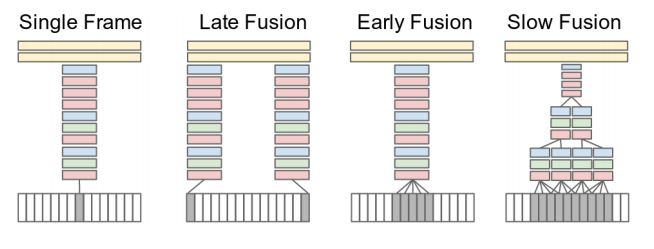
\includegraphics[width=\linewidth]{K_models.JPG}
    \caption{citep{KarpathyCVPR14} explored approaches for fusing information over
    temporal dimension through the network. Red, green and
    blue boxes indicate convolutional, normalization and pooling layers respectively \citep{KarpathyCVPR14}}
    \label{fig:k_models}
\end{figure}
There is a wide range of a pretrained convolution neural networks architectures particularly models for image classification trained on ImageNet dataset on the keras API. However there where a few explored as listed below.
\begin{itemize}
    \item VGG19: as described in \citep{simonyan2014deep}, is quite a standard architecture that is made of a convolutional $3 \times3$ filters with a stride 2, followed by a $2\times2$ max-pool with a stride of 2.
    \item MobileNetV2: is a model created for mobile vision application available in keras. MobileNetV2\cite{Sandler_2018} makes an improvment from its predecessor MobileNetV1 \citep{howard2017mobilenets}, which uses depthwise separable convolution as efficient building blocks. However it introduces a linear bottlenecks between the layers, and a shortcut connections between the bottlenecks.
    \item Inception: this architecture \citep{Szegedy_2016} is made up of inception blocks which evaluate multiple multiple pooling layers of different dimensions then concatenate the results.
    \item ResNet: this architecture \citep{He_2016} is made up of residual blocks, which are a set of two layers that rather than going through the standard path of going from one activation layer to the next, addes the linear equation used to arrive at the activation value for the next layer. This is believed to have the benefit of helping with vanishing and exploding gradients to improve performance as the neural network gets deeper
\end{itemize}
